%Larger RHIRL horizon can allow for more temporally abstract norms to be encoded 
%ex: "pass on the left" may take multiple steps to coordinate and give a reward when agents pass each other on the left

%\vspace{\up}
\paragraph{Norm Learning Results}
\label{sec:results}

We now present preliminary results demonstrating that both our batch
and interactive norm learning algorithms can produce reasonable
results in grid games. For batch learning, we hard code examples of
agents following different norms, and show that our algorithm is able
to recover the appropriate norm when it is trained on demonstrations
of behavior following that norm. We also show that the learned norm
can generalize to sensible behavior in other situations by testing the
agents in similar grid games after learning. For interactive learning,
we show that two agents playing together can very quickly 
%(typically after one round) 
establish a norm, and that restarting learning from scratch can result
in the agents establishing different norms.

For both sets of experiments, we examine behavior in Hallway.  The
social reward function consists of a total welfare team reward
function and a linear family of bias functions. The bias functions
operate on 50 state-joint action binary features. The first 25
features are an indicator variable for selecting one of the 25 joint
actions when the agents are in {\em conflict} and the latter 25
features are indicator functions for selecting one of the 25 joint
actions for when the agents are not a conflict. We define the agents
to be in conflict when they are in the same row of the grid and each
is closer to their opponent's goal than they are to their own
goal. Additionally, when one of the agents is one step away from their
goal, none of the features activate, thereby preventing norm
preferences from favoring premature termination of the joint
task. Since these features directly encode preferences for joint
actions rather than higher-level goals, when training we use RHIRL
with a horizon of 1. We do not expect this set of features to be
complete or capable of capturing all the possible norms that might be
established in a grid game. So an important area for future work is to
identify expressive features that can also generalize
well. Nevertheless, the features used here provide a proof of concept
for our approach.
%which can later be extended to more expressive features.

%\subsection{Batch Training Results}

\begin{figure}
    \centering
    \begin{subfigure}[b]{0.275\textwidth}
        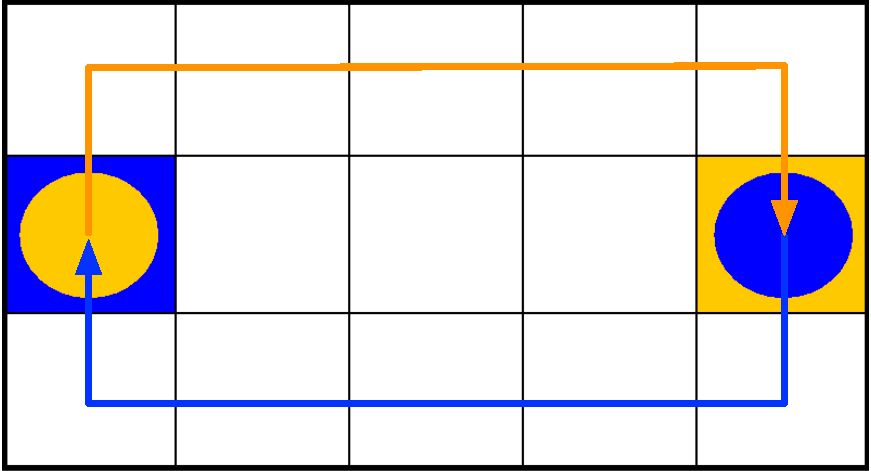
\includegraphics[width=\textwidth]{figures/batch1}
        \caption{}
        \label{fig:batch1}
    \end{subfigure}
\qquad
    ~ %add desired spacing between images, e. g. ~, \quad, \qquad, \hfill etc. 
      %(or a blank line to force the subfigure onto a new line)
    \begin{subfigure}[b]{0.275\textwidth}
        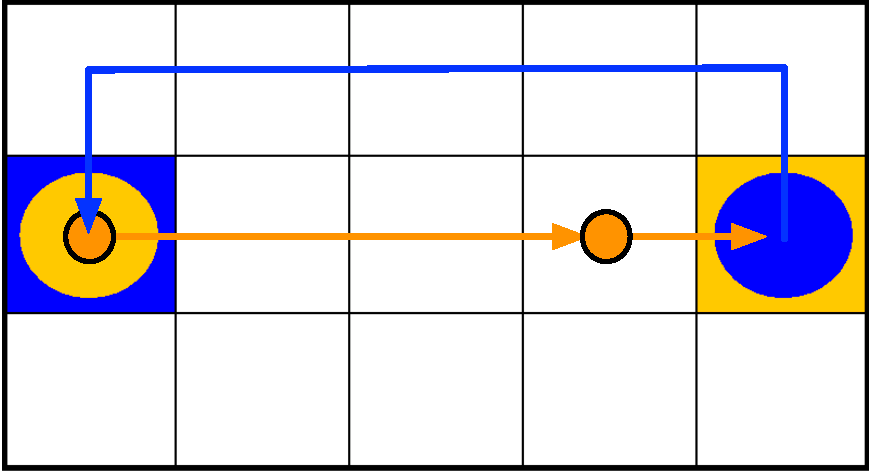
\includegraphics[width=\textwidth]{figures/batch2}
        \caption{}
        \label{fig:batch2}
    \end{subfigure}
\qquad
    ~ %add desired spacing between images, e. g. ~, \quad, \qquad, \hfill etc. 
    %(or a blank line to force the subfigure onto a new line)
    \begin{subfigure}[b]{0.275\textwidth}
        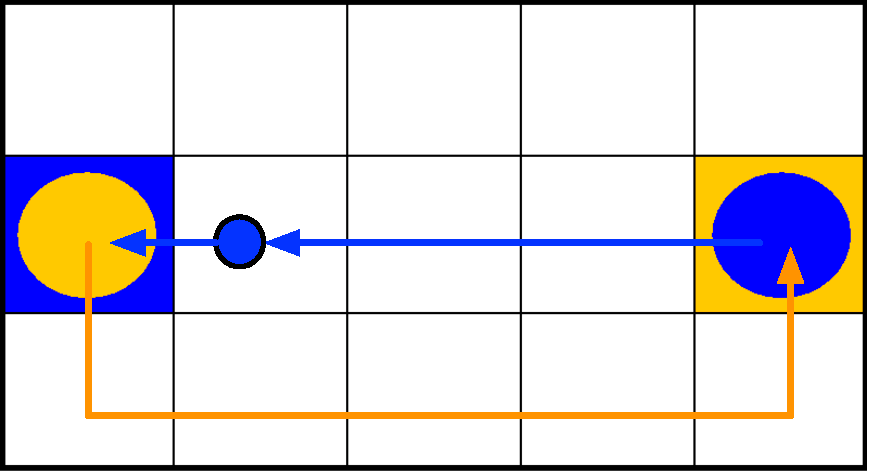
\includegraphics[width=\textwidth]{figures/batch3}
        \caption{}
        \label{fig:batch3}
    \end{subfigure}
    \caption{The three different norms the batch learning algorithm trained on in Hallway. Colored arrows indicate the path of the player of the same color. A small circle indicates a wait action.}\label{fig:batchRes}
\end{figure}

We tested our batch learning algorithm on datasets in which
agents followed three different norms. 
%All three norms are shown in \ref{fig:batchRes}. 
The first norm (Figure~\ref{fig:batch1}) shows the orange player going
north and then along the top row of the grid while the blue player
goes south and then along the bottom row. The second norm
(Figure~\ref{fig:batch2}) shows the blue player going north and along
the top row while the orange player waits, then goes east, and then
waits again for blue to catch up so they can enter their goals
together.  The third norm (Figure~\ref{fig:batch3}) has the orange
player go south and along the bottow row while the blue player
immediately goes west toward its goal and then waits two steps.
%for orange to catch up so they can enter their goals together.

For each of these three norms we generated five demonstrations, two of
which described the norm exactly, and the other three of which
contained slight deviations from the norm (for example, moving back to
the center row before reaching the end). We then
separately trained our batch algorithm on each set of demonstrations.
In all cases, the learned social reward function motivated
behavior that consistently replicated the observed norm on which it
was trained. Additionally, we planned using the learned social reward
function in a larger 7x3 hallway grid game, and obtained the same norm
behavior.

%\subsection{Interactive Training}
%\jmnote{I will also try to run an experiment in which one player is initially biased to show that the other agent adapts to them.}

\begin{figure}
    \centering
    \begin{subfigure}[b]{0.18\textwidth}
        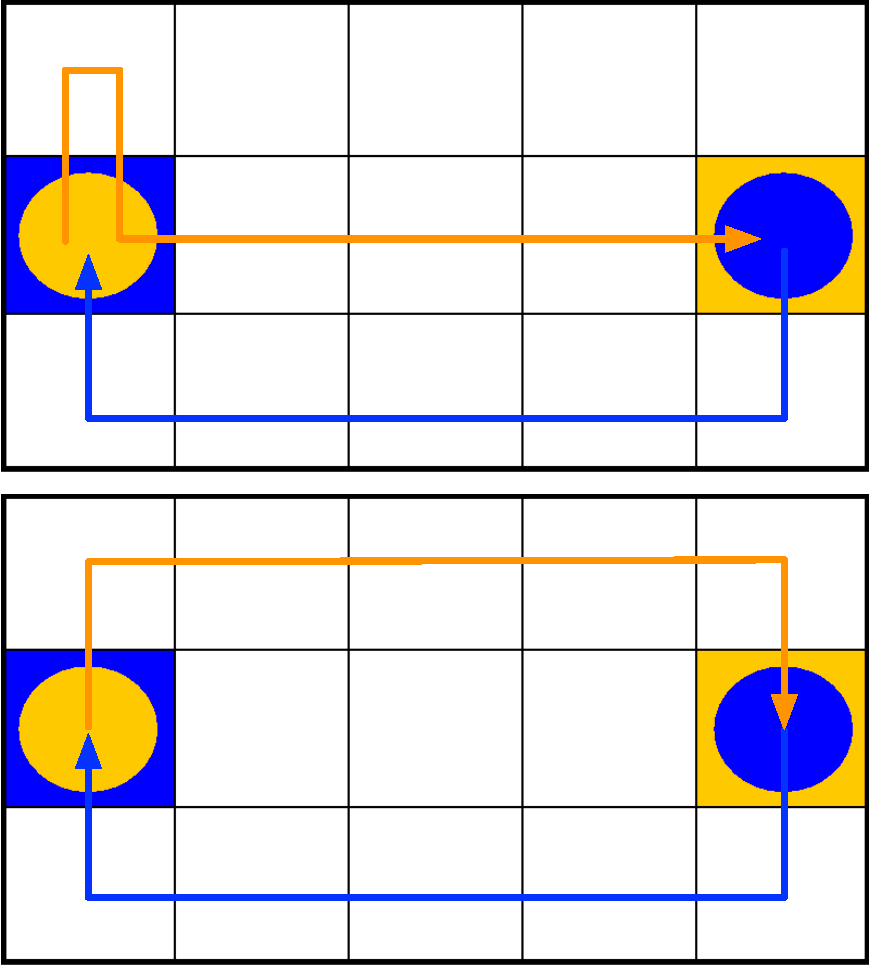
\includegraphics[width=\textwidth]{figures/interactive1}
        \caption{}
        \label{fig:inter1}
    \end{subfigure}
    ~ %add desired spacing between images, e. g. ~, \quad, \qquad, \hfill etc. 
      %(or a blank line to force the subfigure onto a new line)
    \begin{subfigure}[b]{0.18\textwidth}
        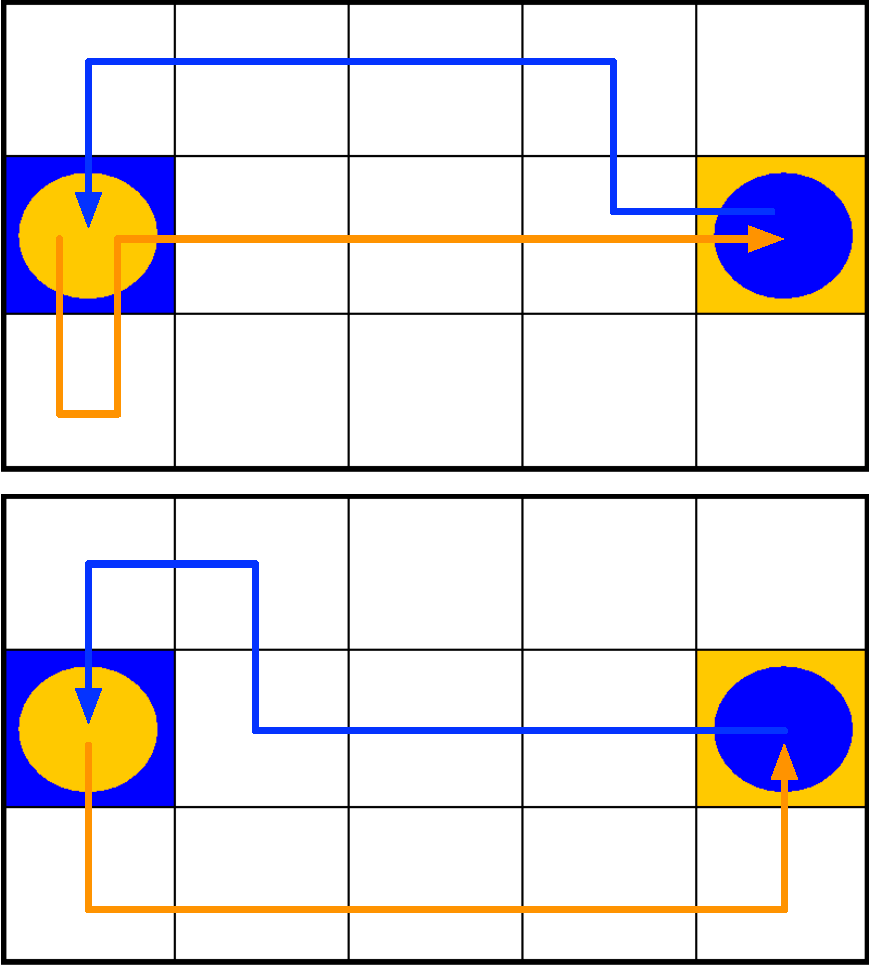
\includegraphics[width=\textwidth]{figures/interactive2}
        \caption{}
        \label{fig:inter2}
    \end{subfigure}
    ~ %add desired spacing between images, e. g. ~, \quad, \qquad, \hfill etc. 
    %(or a blank line to force the subfigure onto a new line)
    \begin{subfigure}[b]{0.18\textwidth}
        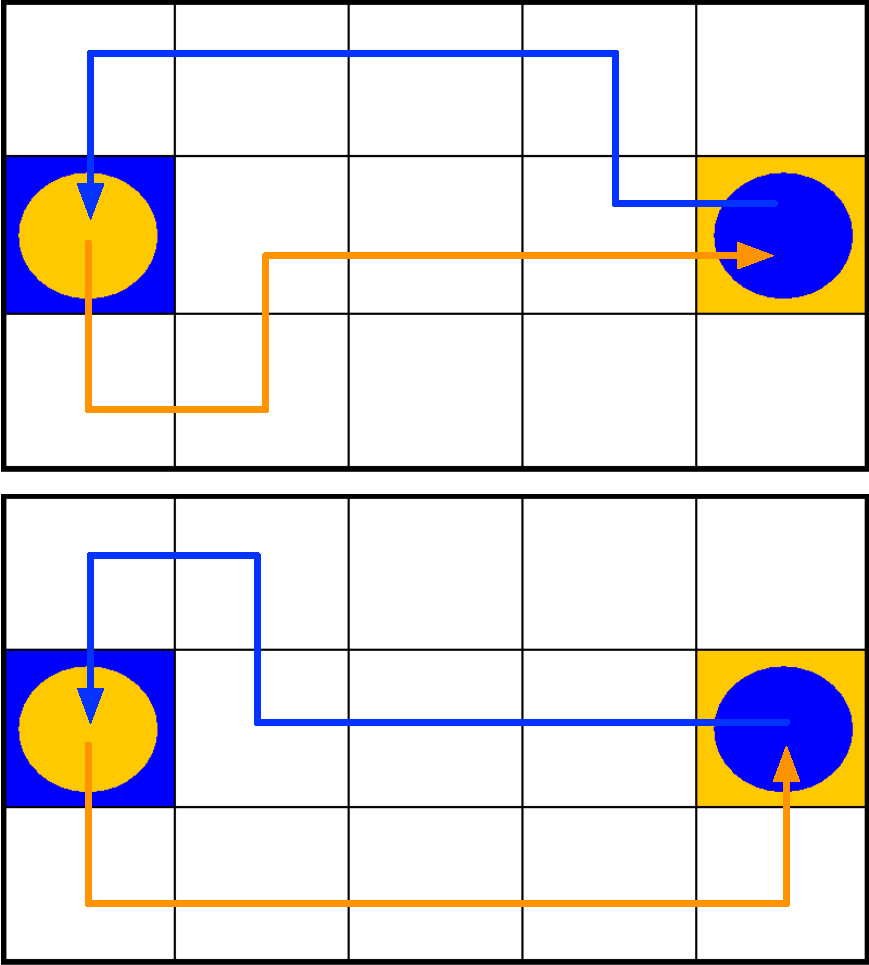
\includegraphics[width=\textwidth]{figures/interactive3}
        \caption{}
        \label{fig:inter3}
    \end{subfigure}
	~ %add desired spacing between images, e. g. ~, \quad, \qquad, \hfill etc. 
    %(or a blank line to force the subfigure onto a new line)
    \begin{subfigure}[b]{0.18\textwidth}
        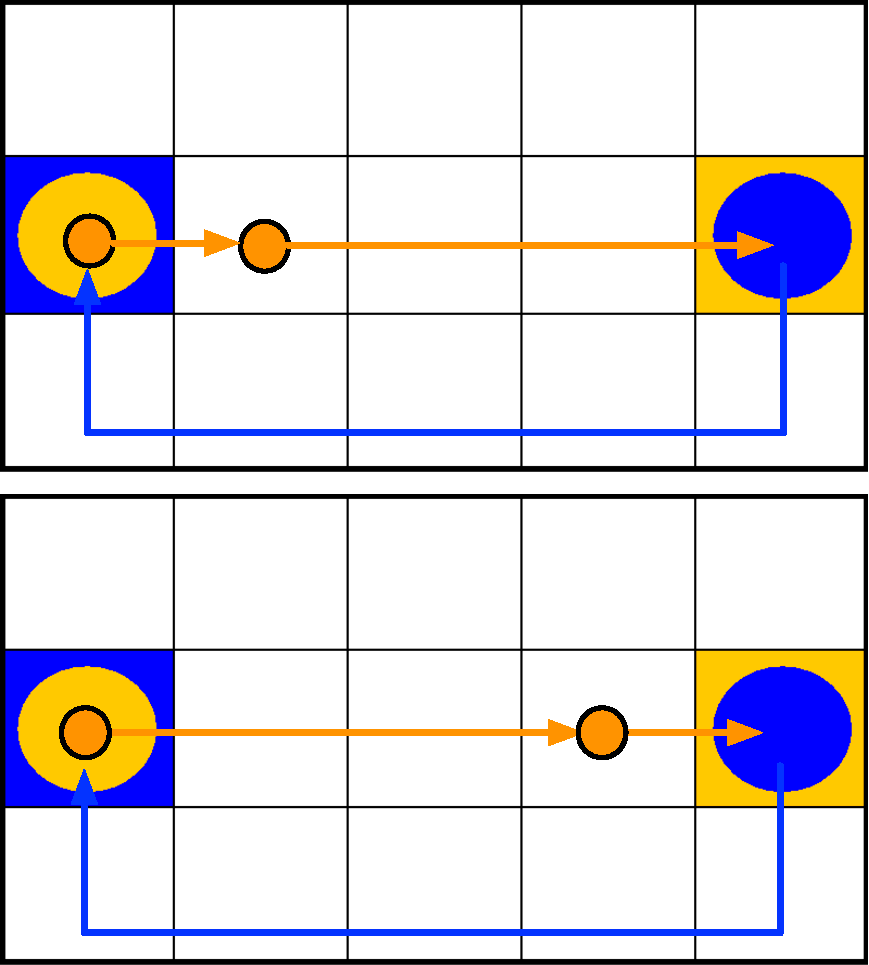
\includegraphics[width=\textwidth]{figures/interactive4}
        \caption{}
        \label{fig:inter4}
    \end{subfigure}
    ~ %add desired spacing between images, e. g. ~, \quad, \qquad, \hfill etc. 
    %(or a blank line to force the subfigure onto a new line)
    \begin{subfigure}[b]{0.18\textwidth}
        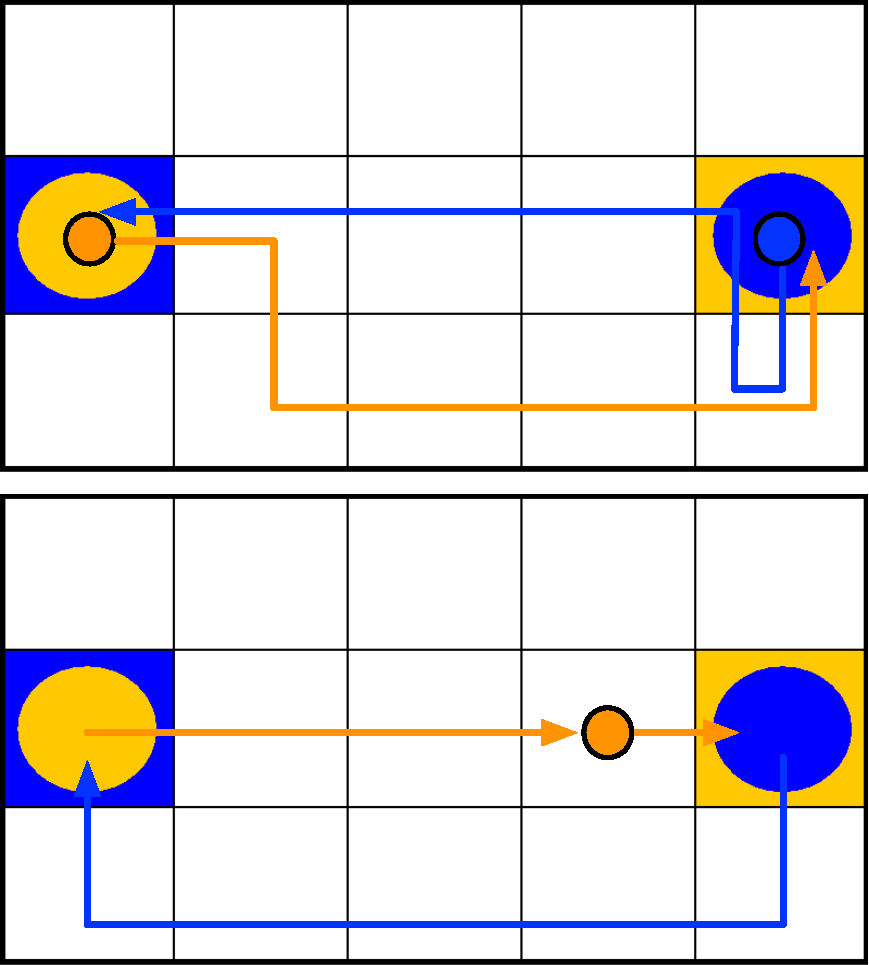
\includegraphics[width=\textwidth]{figures/interactive5}
        \caption{}
        \label{fig:inter5}
    \end{subfigure}
    \caption{The learning results from each of the 5 interactive matches (a-e). The top image for a match is the first round of interaction of the agents. The bottom image for a match is the learned behavior. For matches b-e, the last move of an agent that reaches their goal sooner may be to wait for two steps, or to move north and/or south and back again; only one example is illustrated.}\label{fig:interRes}
\end{figure}

In our interactive norm learning experiment,
%(see Figure~\ref{fig:interRes}), 
we played two interactive learning agents against one another.  The
agents played five matches, each one consisting of five rounds.  Each
match began fresh, without any knowledge of previous matches, to see
whether different norms could emerge.  The social reward function was
initialized to the total welfare joint policy.  In each match, the
agents very quickly (typically after the first round) converged on a
norm that persisted for the rest of the match.  However, in each
match, a different norm was learned, showing that agents employing our
algorithm quickly adapt to the particular shared experience they have
with other agents.
%, and then maintain the learned norm.

Figure~\ref{fig:interRes} shows the results of learning in each of the
five matches (with the top image showing the behavior in the first
round and the bottom image showing the learned behavior). While
different normative behavior was learned in different matches, once
learned, the learned behavior was consistently employed in all
subsequent rounds.  Of particular interest are the results in the
fifth match (Figure~\ref{fig:inter5}). In the first round of this
match, both players wait (a suboptimal joint action), and Blue then
moves in an odd looping motion. Nevertheless, a norm based on the
actions that ultimately worked is learned from the experience, and the
agents do better after that.
